% Provenance (never printed): see sources/outline_sources.md (Year 1: physical and chemical
% weathering; hydrolysis and its degrees; the ionic-potential diagram; clay minerals and
% climate; silicate weathering and carbon dioxide). Exercise and problem values in the Book 3
% scratch calculator calc/ch19.py; figure data from figdata/bachelor-1/ionic_potential.py and
% hydrolysis.py. Weathering is owned by Book 1 g5; chemical weathering, hydrolysis, clay mineral
% and laterite by Book 2 g10 (re-founded here). Silicate classes and the feldspars by ch. 7;
% Bowen's series by Book 2 g11; acid--base chemistry, solubility and oxidation by the chemistry
% books; soils and their horizons by the biology books. The silicate-weathering thermostat
% belongs to the Year 2 volume (told).
\chapter{L'altération et les argiles}\label{ch:b1:weathering-clays}

Les lettres d'une vieille pierre tombale s'effacent, les arêtes vives des lettres
s'arrondissant en rainures peu profondes, plus vite sur une pierre de marbre que sur une d'ardoise.
Un \omterm{def:b1:geological-maps:geological-map}{affleurement} de granite qui paraît aussi dur que n'importe quoi sur Terre s'effrite
en surface en un sable graveleux, qui coule entre les doigts en grains libres
de quartz vitreux, de \omterm{def:b1:rock-forming-minerals:groups}{feldspath} crayeux et de paillettes de \omterm{def:b1:rock-forming-minerals:groups}{mica}. Sous les forêts des
tropiques humides, la roche saine peut se trouver loin en dessous, sous une terre rouge
qui garde les contours des minéraux de la roche mais se coupe à la bêche.
Les trois sont l'œuvre de l'eau à la surface de la Terre. Ce chapitre écrit
cette œuvre comme de la chimie~: quels minéraux cèdent les premiers, ce qu'ils deviennent, pourquoi
certains éléments partent avec l'eau et d'autres restent, comment le climat fixe
le résultat, et comment la lente décomposition de la roche silicatée tire le dioxyde de carbone
de l'air.

\begin{recall}
L'altération brise les roches là où elles se trouvent (livre~1, année~5). L'\omterm{def:b1:weathering-clays:weathering}{altération
chimique} transforme les minéraux~; l'\omterm{def:b1:weathering-clays:hydrolysis}{hydrolyse} d'un \omterm{def:b1:rock-forming-minerals:groups}{feldspath} donne un \omterm{def:b1:weathering-clays:clay-mineral}{minéral
argileux}, la \omterm{def:b1:weathering-clays:clay-mineral}{kaolinite}, et envoie du potassium et de la silice aux rivières~; une \omterm{def:b1:weathering-clays:laterite}{latérite} est
le produit rouge, riche en fer et en aluminium, des climats chauds et humides (livre~2,
année~10). Les silicates sont classés selon la façon dont leurs tétraèdres \ce{SiO4} partagent
leurs sommets, un \omterm{def:b1:rock-forming-minerals:silicate-classes}{phyllosilicate} formant des feuillets~; les \omterm{def:b1:rock-forming-minerals:groups}{feldspaths} sont des silicates en charpente de
sodium, de potassium et de calcium, les \omterm{def:b1:rock-forming-minerals:groups}{micas} des silicates en feuillets avec du potassium entre les
feuillets (\cref{def:b1:rock-forming-minerals:silicate-classes},
\cref{def:b1:rock-forming-minerals:groups}). Le rayon ionique d'un ion dépend de
sa charge et de sa coordinence (\cref{ch:b1:rock-forming-minerals}). Les minéraux
cristallisent d'un magma qui se refroidit dans l'ordre de la série de réaction de Bowen,
l'\omterm{def:b1:rock-forming-minerals:groups}{olivine} d'abord et le quartz en dernier (livre~2, année~11). Un acide libère des
ions hydrogène~; le dioxyde de carbone dissous dans l'eau forme de l'acide carbonique~; une oxydation est une
perte d'électrons~; une équation équilibrée conserve chaque élément et la charge
(livres de chimie). Un sol est une couche vivante organisée en horizons (livres de
biologie).
\end{recall}

\section{Altération physique et chimique}\label{sec:b1:weathering-clays:types}

Une roche formée en profondeur, à haute température et pression et sans eau libre
ni oxygène, est hors d'équilibre à la surface. Elle s'ajuste de deux façons, qui
agissent ensemble.

\begin{definition}[Altération physique, altération chimique]\label{def:b1:weathering-clays:weathering}
L'\emph{altération physique}\index{alteration physique@altération physique} est la désagrégation d'une
roche en place en fragments plus petits sans changement de ses minéraux.
L'\emph{altération chimique}\index{alteration chimique@altération chimique} est la transformation des
minéraux d'une roche en place par réaction avec l'eau et les substances qu'elle
transporte, surtout les ions hydrogène, le dioxyde de carbone dissous et l'oxygène~: certains
minéraux se dissolvent, d'autres sont remplacés par de nouveaux minéraux stables en surface,
et une partie de la roche part en solution.
\end{definition}
% ledger: formoso:weathering

\emph{Le gel.} L'eau à \qty{0}{\celsius} a pour masse volumique
\qty{999.87}{kg.m^{-3}}, la glace \qty{916.72}{kg.m^{-3}}~: l'eau se dilate de
\qty{9.1}{\percent} en gelant. L'ancienne image de la gélifraction est
de l'eau gelant dans une fissure close et la forçant à s'ouvrir, de nouveau à chaque dégel et
chaque gel. Un modèle de fissures dans le granite et le marbre, bâti sur la mécanique de la rupture
et sur ce que l'on sait des sols qui gèlent, met l'accent ailleurs~: l'eau est
attirée à travers les pores vers la glace déjà présente dans une fissure, comme elle l'est vers les
lentilles de glace d'un sol qui gèle, et la glace grossit et coince la fissure tant que
dure le gel. Un gel prolongé est le plus efficace entre environ
\qty{-4}{\celsius} et \qty{-15}{\celsius}~: plus près de zéro la glace ne peut
accumuler assez de pression, et plus froid l'eau ne peut plus s'y déplacer.
% ledger: usgs:water-density, iapws:ice-density, wh85:frost

\emph{Chauffage, décharge et sel.} Des chauffages et refroidissements répétés fatiguent une
roche dont les minéraux se dilatent de quantités différentes~; un granite amené à la
surface par l'érosion, délesté du poids au-dessus de lui, se dilate et se fend en
feuillets parallèles à la surface~; des sels cristallisant d'une eau qui s'évapore,
dans les déserts et sur les côtes, écartent les grains.

L'\omterm{def:b1:weathering-clays:weathering}{altération physique} fait plus que briser la roche~: elle l'ouvre à l'eau.

\begin{proposition}[La surface ouverte par la fragmentation]\label{prop:b1:weathering-clays:surface}
Un cube de côté $L$ découpé en cubes de côté $L/n$ a $n$ fois l'aire de
surface. Plus généralement, une masse $m$ de grains de masse volumique $\rho$, tous cubes de côté
$d$, a l'aire de surface $S = 6m/(\rho d)$~: la surface spécifique $S/m =
6/(\rho d)$ est inversement proportionnelle à la taille des grains.
\end{proposition}

\begin{proof}
Un cube de côté $d$ a l'aire $6d^2$ et la masse $\rho d^3$, donc la
surface spécifique de chaque grain, et de n'importe quel nombre d'entre eux, est $6d^2/(\rho d^3)
= 6/(\rho d)$. Découper un cube de côté $L$ en $n^3$ cubes de côté $L/n$ conserve
la masse et divise $d$ par $n$, ce qui multiplie l'aire par $n$.
\end{proof}

Un bloc de \omterm{def:b1:rock-forming-minerals:groups}{feldspath} de masse volumique environ \qty{2600}{kg.m^{-3}} a une surface
spécifique de \qty{0.23}{m^2.kg^{-1}} en fragments centimétriques, et
\qty{2.3}{m^2.g^{-1}} en grains micrométriques, dix mille fois plus. Les réactions
chimiques se font aux surfaces, donc une roche fracassée par le gel ou ouverte le long de
ses joints s'altère chimiquement bien plus vite que la même roche intacte.
% ledger: hom:albite, hom:orthoclase

\emph{Les réactions chimiques.} La calcite se dissout complètement dans l'eau qui
transporte du dioxyde de carbone, ce qui explique que les pierres tombales de marbre perdent leurs lettres
(livre~2, année~10). Le fer(II) des silicates sombres est oxydé en fer(III),
qui reste sous forme d'oxydes jaune-brun et rouges. Le plus important de loin, parce que
les silicates font l'essentiel de la \omterm{def:b1:layered-earth:layers}{croûte}, est l'\omterm{def:b1:weathering-clays:hydrolysis}{hydrolyse}. Les ions hydrogène viennent du
dioxyde de carbone, dissous depuis l'air et expiré par les racines et les
décomposeurs dans le sol, et des acides organiques des plantes en décomposition~:
les eaux de surface et de sol non polluées ont un pH entre 5.5 et 7, et l'eau
de la couche organique de certains sols forestiers aussi bas que 3.5. L'eau, la température,
la surface et l'acidité sont ainsi les quatre contrôles de l'\omterm{def:b1:weathering-clays:weathering}{altération chimique},
et un climat chaud et humide avec un sol épais fournit les quatre.
% ledger: formoso:weathering

\section{L'hydrolyse des silicates}\label{sec:b1:weathering-clays:hydrolysis}

\begin{definition}[Hydrolyse d'un silicate]\label{def:b1:weathering-clays:hydrolysis}
L'\emph{hydrolyse}\index{hydrolyse (des silicates)} d'un silicate est sa
réaction avec l'eau et les ions hydrogène, dans laquelle les ions hydrogène remplacent les
cations métalliques, qui passent en solution, une partie ou la totalité du silicium part sous forme
d'acide silicique dissous \ce{H4SiO4}, et le reste du \omterm{def:b1:rock-forming-minerals:mineral}{minéral} est reconstruit en
un nouveau solide, un \omterm{def:b1:weathering-clays:clay-mineral}{minéral argileux} ou un hydroxyde. La dissolution est incongruente~:
le solide restant n'a pas la composition du \omterm{def:b1:rock-forming-minerals:mineral}{minéral} attaqué.
\end{definition}
% ledger: formoso:weathering

L'aluminium est la clé pour écrire la réaction~: au pH des sols et des rivières il
est presque insoluble, et le produit solide le garde tout entier. Tout le reste
en découle.

\begin{method}[Équilibrer une réaction d'hydrolyse]\label{met:b1:weathering-clays:balance}
Étant donnés le \omterm{def:b1:rock-forming-minerals:mineral}{minéral} attaqué et le produit solide~:
\begin{enumerate}
  \item Prendre une unité formulaire du produit, et autant de \omterm{def:b1:rock-forming-minerals:mineral}{minéral} qu'il en faut pour
        apporter le même nombre d'atomes d'aluminium.
  \item Le silicium du \omterm{def:b1:rock-forming-minerals:mineral}{minéral} non utilisé par le produit part sous forme de
        \ce{H4SiO4}~; les cations métalliques non utilisés par le produit partent sous forme d'ions.
  \item Équilibrer la charge de ces cations avec des ions hydrogène à gauche.
  \item Équilibrer l'oxygène avec de l'eau à gauche.
  \item Vérifier l'hydrogène~: il doit s'équilibrer de lui-même. S'il ne le fait pas, une
        formule est fausse.
  \item Si une équation à nombres entiers est voulue, multiplier le tout.
\end{enumerate}
\end{method}

\begin{proposition}[Hydrolyse des feldspaths]\label{prop:b1:weathering-clays:feldspars}
Avec la \omterm{def:b1:weathering-clays:clay-mineral}{smectite} beidellite \ce{Na_{0.5}Al2(Si_{3.5}Al_{0.5})O10(OH)2}
(eau interfoliaire omise), la \omterm{def:b1:weathering-clays:clay-mineral}{kaolinite} \ce{Al2Si2O5(OH)4} et la gibbsite
\ce{Al(OH)3} comme produits,
\begin{align*}
&\ce{5 NaAlSi3O8 + 4 H+ + 16 H2O -> 2 Na_{0.5}Al2(Si_{3.5}Al_{0.5})O10(OH)2 + 4 Na+ + 8 H4SiO4},\\ % ce-unbalanced-ok: decimal subscripts the checker cannot read; balance tested in tests/bachelor-1/test_weathering_clays.py
&\ce{2 NaAlSi3O8 + 2 H+ + 9 H2O -> Al2Si2O5(OH)4 + 2 Na+ + 4 H4SiO4},\\
&\ce{NaAlSi3O8 + H+ + 7 H2O -> Al(OH)3 + Na+ + 3 H4SiO4},\\
&\ce{CaAl2Si2O8 + 2 H+ + H2O -> Al2Si2O5(OH)4 + Ca^2+}.
\end{align*}
L'albite perd \qty{80}{\percent} de son sodium et $8/15$ de son silicium dans
la solution dans la première réaction, tout son sodium et $2/3$ de son silicium dans
la deuxième, la totalité des deux dans la troisième. L'anorthite perd tout son calcium et
aucun silicium.
\end{proposition}
% ledger: webmineral:clays-b19, hom:albite, hom:anorthite

\begin{proof}
Appliquons la méthode. Première réaction~: deux unités de beidellite contiennent $2\times2.5 = 5$
aluminium, l'aluminium de 5 albite~; les 15 silicium de l'albite moins les
$2\times3.5 = 7$ du produit donnent 8 \ce{H4SiO4}~; les 5 sodium moins 1 donnent
4 \ce{Na+}, équilibrés par 4 \ce{H+}~; l'oxygène, $40 + w$ à gauche et $24 + 32 =
56$ à droite, donne $w = 16$~; l'hydrogène, $4 + 32 = 36$ et $4 + 32 = 36$,
se vérifie. Deuxième~: 2 albite donnent les 2 aluminium de la \omterm{def:b1:weathering-clays:clay-mineral}{kaolinite}, $6 - 2 = 4$
\ce{H4SiO4}, 2 \ce{Na+} et 2 \ce{H+}~; l'oxygène $16 + w = 9 + 16$ donne $w = 9$~;
l'hydrogène $2 + 18 = 20 = 4 + 16$. Troisième~: une albite, trois acides siliciques, un
\ce{Na+} et un \ce{H+}~; l'oxygène $8 + w = 3 + 12$ donne $w = 7$~; l'hydrogène
$1 + 14 = 15 = 3 + 12$. Quatrième~: les 2 aluminium et 2 silicium de l'anorthite sont
exactement ceux de la \omterm{def:b1:weathering-clays:clay-mineral}{kaolinite}, aucun acide silicique ne part, \ce{Ca^2+} demande 2 \ce{H+}~;
l'oxygène $8 + w = 9$ donne $w = 1$~; l'hydrogène $2 + 2 = 4$. Les fractions
exportées sont les ions en solution sur les atomes dans le \omterm{def:b1:rock-forming-minerals:mineral}{minéral}~: $4/5$ et $8/15$, puis
$2/2$ et $4/6$, puis $1/1$ et $3/3$.
\end{proof}

La même albite peut donc donner trois solides différents, et celui qu'elle donne
dépend de la quantité d'eau qui traverse la roche et emporte les produits~:
peu d'eau, et une grande part de la silice et quelques cations restent pour
construire une \omterm{def:b1:weathering-clays:clay-mineral}{smectite}~; davantage, et seule assez de silice pour la \omterm{def:b1:weathering-clays:clay-mineral}{kaolinite} reste~; beaucoup
d'eau, et la silice part entièrement.

\begin{definition}[Bisiallitisation, monosiallitisation, allitisation]\label{def:b1:weathering-clays:hydrolysis-degree}
Le degré d'\omterm{def:b1:weathering-clays:hydrolysis}{hydrolyse} des silicates est nommé d'après son produit.
La \emph{bisiallitisation}\index{bisiallitisation} forme des minéraux argileux 2:1, comme les
\omterm{def:b1:weathering-clays:clay-mineral}{smectites}, avec environ deux atomes de silicium par aluminium~; une partie des cations
reste en eux. La \emph{monosiallitisation}\index{monosiallitisation} forme des
minéraux argileux 1:1, la \omterm{def:b1:weathering-clays:clay-mineral}{kaolinite}, avec un silicium par aluminium~; tous les cations alcalins et
alcalino-terreux partent. L'\emph{allitisation}\index{allitisation} retire
entièrement le silicium et laisse de l'hydroxyde d'aluminium, la gibbsite.
\end{definition}
% ledger: pedron:stages, formoso:weathering

Le degré atteint dépend d'abord du climat, par la pluie et la
température, puis du drainage du profil. Là où l'eau est
peu renouvelée, un granite perd une grande part de son sodium et de son calcium, son potassium plus
lentement, et seulement une part de sa silice~: ses \omterm{def:b1:rock-forming-minerals:groups}{feldspaths} se transforment en argiles 2:1, et
beaucoup de quartz reste~; la roche se désagrège en un sable de quartz, de \omterm{def:b1:rock-forming-minerals:groups}{mica} et de
\omterm{def:b1:rock-forming-minerals:groups}{feldspath} à demi altéré mêlé d'argile. Sous les fortes pluies des
tropiques humides, plus de \qty{2000}{mm} par an, les cations et la silice sont
lessivés bien davantage, et la \omterm{def:b1:weathering-clays:clay-mineral}{kaolinite}, Si/Al = 1, se forme. Là où le lessivage est le plus
intense, même la silice de la \omterm{def:b1:weathering-clays:clay-mineral}{kaolinite} part, et la gibbsite reste.
% ledger: pedron:stages, goldich:1938, formoso:laterite

\begin{omfigure}
\begin{tikzpicture}[font=\small]
% fractions of albite's Na and Si exported by the three degrees (figdata/bachelor-1/hydrolysis.py)
\begin{axis}[width=10.5cm, height=6cm, ybar, bar width=0.5cm, ymin=0, ymax=112,
    xmin=0.45, xmax=3.55, xtick={1,2,3},
    xticklabels={{bisiallitisation\\ vers la beidellite\\ (Si/Al = 1.4)}, {monosiallitisation\\ vers la kaolinite\\ (Si/Al = 1)}, {allitisation\\ vers la gibbsite\\ (Si/Al = 0)}},
    xticklabel style={align=center, font=\footnotesize},
    ylabel={exporté en solution (\si{\percent})}, ytick={0,20,...,100},
    legend style={at={(0.5,1.03)}, anchor=south, font=\footnotesize, legend columns=2, draw=none},
    nodes near coords={\pgfmathprintnumber[fixed,precision=0]{\pgfplotspointmeta}}, every node near coord/.append style={font=\scriptsize},
    enlarge x limits=false]
  \addplot[fill=omThm!60, draw=omThm!80!black] table[x=degree, y=Na] {figdata/out/bachelor-1-hydrolysis-degrees.dat};
  \addplot[fill=omDef!55, draw=omDef!80!black] table[x=degree, y=Si] {figdata/out/bachelor-1-hydrolysis-degrees.dat};
  \legend{sodium, silicium}
\end{axis}
\end{tikzpicture}

{\small Les trois degrés d'\omterm{def:b1:weathering-clays:hydrolysis}{hydrolyse} de l'albite~: le pourcentage de son sodium
et de son silicium emporté en solution, calculé à partir des réactions équilibrées,
et le rapport silicium sur aluminium du solide restant. L'aluminium
reste entièrement dans le solide dans les trois cas.}
\label{fig:b1:weathering-clays:degrees}
\end{omfigure}


\begin{omfigure}
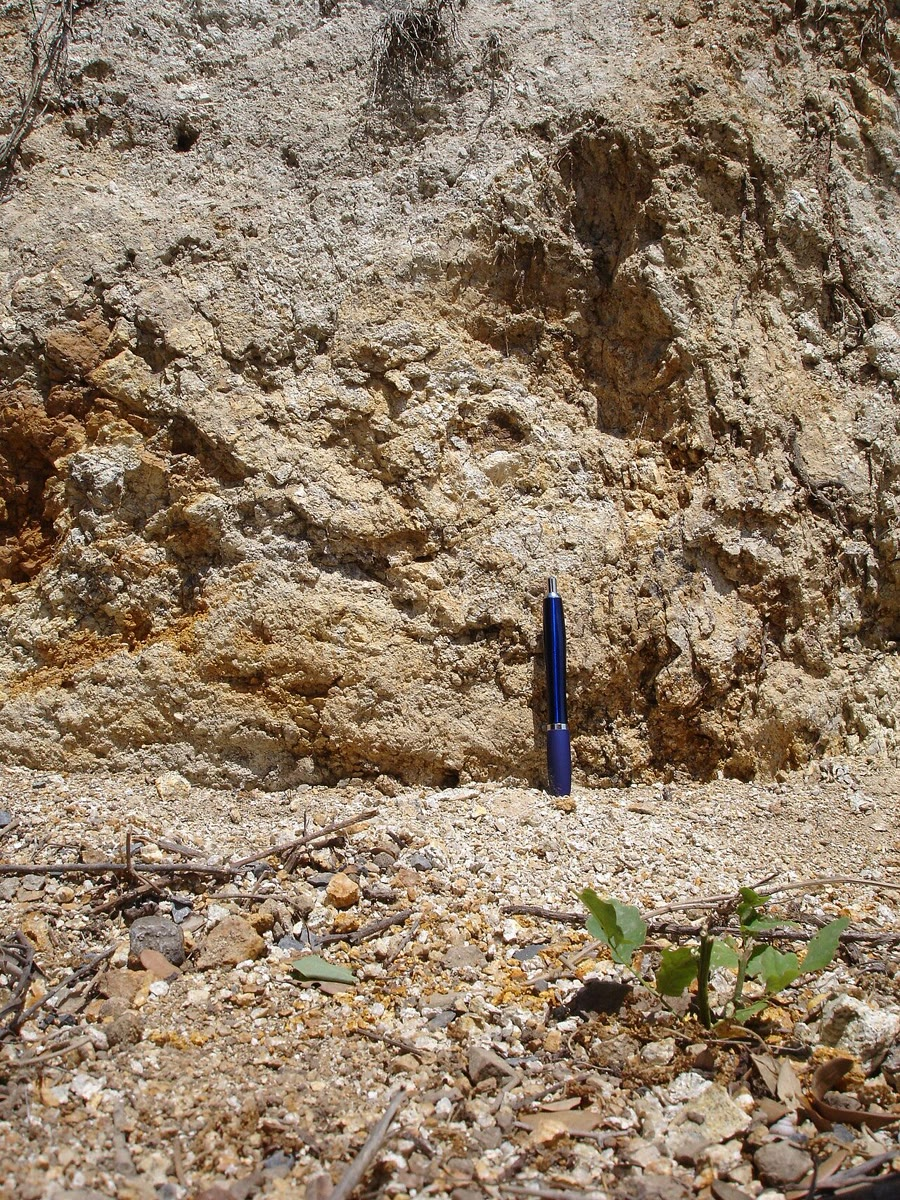
\includegraphics[height=6.3cm]{images/book3/b1-granite-grus.jpg}\hfill
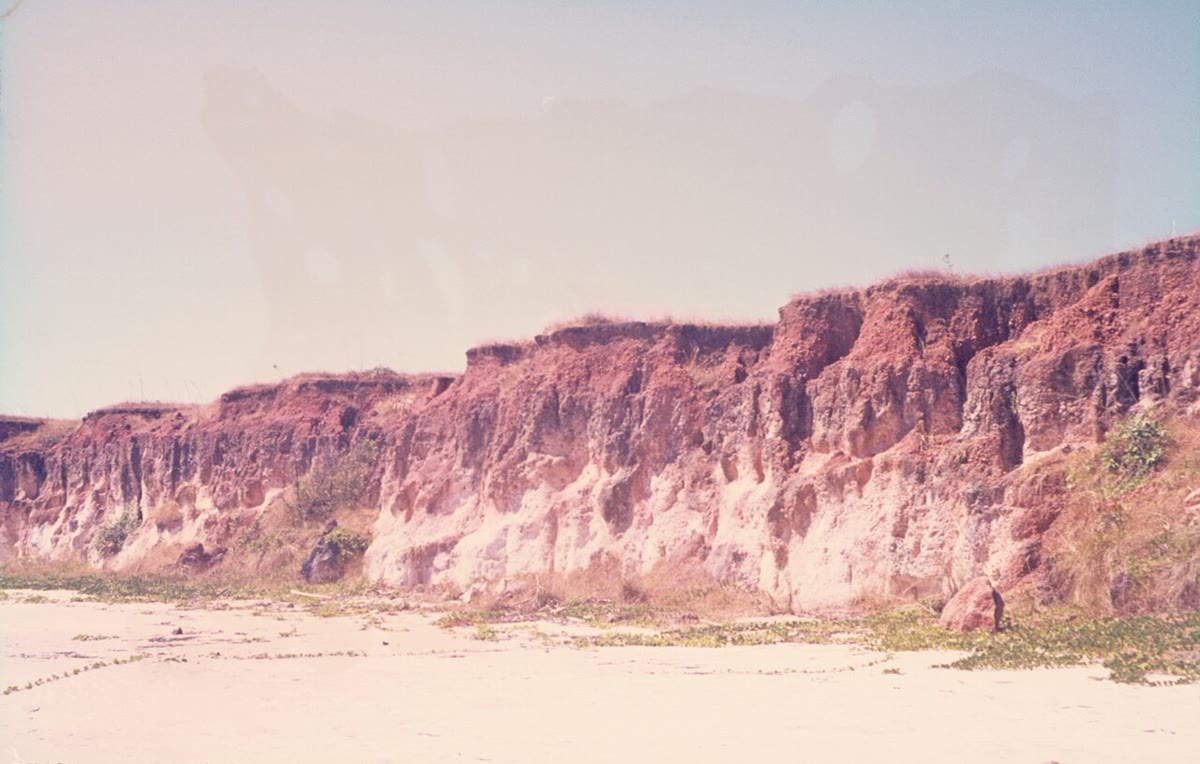
\includegraphics[height=6.3cm]{images/book3/b1-bauxite-weipa.jpg}
\par\smallskip{\small À gauche~: du granite pourri dans les Pyrénées, encore en place mais
s'effritant en un sable de quartz, de \omterm{def:b1:rock-forming-minerals:groups}{feldspath} et de \omterm{def:b1:rock-forming-minerals:groups}{mica}, avec le sable libre à son
pied~; le stylo donne l'échelle. Photographie~: Pinpin, CC~BY~2.5. À droite~: un
profil d'altération sur la côte à Weipa, dans le nord de l'Australie~: de la bauxite rouge, le
produit de l'\omterm{def:b1:weathering-clays:hydrolysis-degree}{allitisation}, au-dessus d'un grès blanc riche en \omterm{def:b1:weathering-clays:clay-mineral}{kaolinite}. Photographie~:
Werner Schellmann, 1969, CC~BY-SA~2.5. Les deux proviennent de Wikimedia Commons.}
\label{fig:b1:weathering-clays:photos}
\end{omfigure}
% ledger: commons:grus, commons:weipa

\emph{Quels minéraux partent les premiers.} En 1938 Samuel Goldich, comparant des profils
altérés à leurs roches mères, proposa une série des minéraux du
moins au plus stable à l'altération, et trouva qu'elle suit l'ordre
dans lequel ils cristallisent d'un magma~: l'\omterm{def:b1:rock-forming-minerals:groups}{olivine} et le \omterm{def:b1:rock-forming-minerals:groups}{plagioclase} riche en calcium
d'abord, le quartz en dernier. Les minéraux formés aux plus hautes températures sont les
plus loin de l'équilibre à la surface. Une liste moderne, du moins au
plus résistant, se lit~: pyrite, calcite, dolomite, \omterm{def:b1:rock-forming-minerals:groups}{olivine}, \omterm{def:b1:rock-forming-minerals:groups}{plagioclase}
calcique, \omterm{def:b1:rock-forming-minerals:groups}{pyroxènes}, \omterm{def:b1:rock-forming-minerals:groups}{plagioclase} intermédiaire, \omterm{def:b1:rock-forming-minerals:groups}{amphiboles}, biotite,
\omterm{def:b1:rock-forming-minerals:groups}{feldspath} potassique, muscovite, \omterm{def:b1:weathering-clays:clay-mineral}{smectite}, quartz, \omterm{def:b1:weathering-clays:clay-mineral}{kaolinite}, et les oxydes
gibbsite et hématite. Les mesures de laboratoire des vitesses de dissolution confirment
le classement~; cela reste un classement, non une loi, puisque la vitesse de chaque \omterm{def:b1:rock-forming-minerals:mineral}{minéral}
dépend aussi de l'eau qui l'entoure. Les produits finaux de l'altération,
\omterm{def:b1:weathering-clays:clay-mineral}{kaolinite}, gibbsite et hématite, sont les plus résistants de tous~: ils sont
déjà stables à la surface.
% ledger: goldich:1938, formoso:weatherability, lasaga:1984

\emph{Le bilan d'un profil d'altération.} L'altération retire de la matière, donc une
concentration mesurée dans une roche altérée ne dit pas combien a été perdu~:
la perte d'autres éléments concentre ceux qui restent. Un élément qui
ne bouge pas donne la référence.

\begin{proposition}[Bilan de masse avec un élément immobile]\label{prop:b1:weathering-clays:immobile}
Soit $i$ un élément que l'altération ne déplace pas, de fractions massiques
$C_{i,p}$ dans la roche mère et $C_{i,w}$ dans la roche altérée. Alors une masse
$m_p$ de roche mère devient la masse $m_w = m_p C_{i,p}/C_{i,w}$ de roche
altérée, et la fraction de tout autre élément $j$ perdue est
\[
  f_j = 1 - \frac{C_{j,w}}{C_{j,p}}\,\frac{C_{i,p}}{C_{i,w}} .
\]
\end{proposition}

\begin{proof}
La masse de $i$ est conservée~: $m_p C_{i,p} = m_w C_{i,w}$, ce qui donne $m_w$.
La masse de $j$ passe de $m_p C_{j,p}$ à $m_w C_{j,w}$, une fraction
$m_w C_{j,w}/(m_p C_{j,p}) = (C_{j,w}/C_{j,p})(C_{i,p}/C_{i,w})$ en
restant~; $f_j$ est un moins cette fraction.
\end{proof}

Le titane et le zirconium sont les choix habituels, pour une raison que la section suivante
donne.

\section{Quels éléments partent~: le potentiel ionique}\label{sec:b1:weathering-clays:ionic}

Le sodium, le potassium et le calcium partent avec l'eau~; l'aluminium, le fer(III) et
le titane restent~; le silicium est entre les deux. La différence tient à la façon dont chaque ion
se comporte dans l'eau.

\begin{definition}[Potentiel ionique]\label{def:b1:weathering-clays:ionic-potential}
Le \emph{potentiel ionique}\index{potentiel ionique} d'un ion est le rapport $z/r$
de son nombre de charge $z$ à son rayon ionique $r$, ici en ångströms (pour la
même coordinence pour tous les ions, six dans ce qui suit).
\end{definition}
% ledger: nomad:goldschmidt, dangic:goldschmidt, shannon:radii-b19

\begin{proposition}[Les trois domaines du potentiel ionique]\label{prop:b1:weathering-clays:fields}
Dans l'eau de l'altération, les ions avec $z/r < 3$ restent en solution sous forme de
cations hydratés et sont emportés (cations solubles)~; les ions avec $3 < z/r < 10$ lient
les ions hydroxyde de l'eau et précipitent en hydroxydes ou oxydes là où ils
sont libérés (hydrolysats)~; les ions avec $z/r > 10$ lient l'oxygène si fortement
qu'ils repoussent les ions hydrogène et voyagent comme des oxyanions solubles, tels que
carbonate, sulfate, phosphate et nitrate. Le silicium, à $z/r = 10$, se trouve sur la
limite, et est lessivé en partie, d'autant plus que l'altération est intense.
\end{proposition}
\admitted
% ledger: nomad:goldschmidt, dangic:goldschmidt

La règle est empirique, due à Victor Moritz Goldschmidt dans les années 1930, et ses
limites sont approximatives~; la chimie qui la sous-tend, l'attraction entre un
cation et l'oxygène des molécules d'eau qui l'entourent, relève des
livres de chimie. Un petit cation très chargé tire si fort sur les électrons de ses
molécules d'eau qu'elles perdent un ion hydrogène et deviennent hydroxyde~:
modérément, et l'hydroxyde précipite~; extrêmement, et même l'hydroxyde
perd son hydrogène, laissant un oxyanion.

Le diagramme ci-dessous lit d'un coup d'œil l'altération d'une roche. Le sodium ($z/r = 0.98$),
le potassium (0.72), le calcium (2.0) et le magnésium (2.8) partent~: ce sont les
cations de l'eau des rivières et de la mer. L'aluminium (5.6), le fer(III) (4.7), le titane
(6.6) et le zirconium (5.6) restent, et s'accumulent dans les profils les plus altérés~;
le titane et le zirconium, qui de plus se trouvent dans des minéraux qui s'altèrent à peine,
sont les références immobiles de la \cref{prop:b1:weathering-clays:immobile}. Le silicium
(10.0) est l'élément dont la perte partielle définit les degrés d'\omterm{def:b1:weathering-clays:hydrolysis}{hydrolyse}.
% ledger: shannon:radii-b19

L'oxydation fait passer un ion de l'autre côté de la limite. Le fer(II), avec $z/r = 2.6$, est un
cation soluble~; le fer(III), à 4.7, un hydrolysat. Dans un sol gorgé d'eau
sans oxygène, le fer se dissout sous forme de \ce{Fe^2+} et est emporté, laissant un sol
gris~; là où l'eau rencontre l'air, à une source ou dans un sol bien drainé, le
fer est oxydé et précipite aussitôt en oxydes rouges et bruns. Le manganèse
se comporte de la même façon, \ce{Mn^2+} (2.4) contre \ce{Mn^4+} (7.5).
% ledger: nomad:goldschmidt, shannon:radii-b19

\begin{omfigure}
\begin{tikzpicture}[font=\small]
% ionic-potential diagram (figdata/bachelor-1/ionic_potential.py): charge against Shannon radius
\begin{axis}[width=12.5cm, height=8.4cm, xmin=0, xmax=1.8, ymin=0, ymax=7,
    xlabel={rayon ionique $r$ (\si{\angstrom}, coordinence six)}, ylabel={charge $z$},
    ytick={1,...,6}, xtick={0,0.2,...,1.8}, xticklabel style={/pgf/number format/fixed},
    axis on top, clip=true]
  \fill[omThm!14] (axis cs:0,0) -- (axis cs:1.8,0) -- (axis cs:1.8,5.4) -- cycle;
  \fill[omDef!16] (axis cs:0,0) -- (axis cs:1.8,5.4) -- (axis cs:1.8,7) -- (axis cs:0.7,7) -- cycle;
  \fill[omExo!18] (axis cs:0,0) -- (axis cs:0.7,7) -- (axis cs:0,7) -- cycle;
  \addplot[black, thick] table[x=r, y=z3] {figdata/out/bachelor-1-ionic_potential-lines.dat};
  \addplot[black, thick] table[x=r, y=z10] {figdata/out/bachelor-1-ionic_potential-lines.dat};
  \addplot[only marks, mark=*, mark size=1.6pt, black,
      point meta=explicit symbolic, nodes near coords,
      visualization depends on={value \thisrow{anc} \as \anc},
      every node near coord/.append style={font=\scriptsize, inner sep=2.6pt, anchor=\anc}]
    table[x=r, y=z, meta=tex] {figdata/out/bachelor-1-ionic_potential-ions.dat};
  \node[font=\footnotesize, align=center, fill=white, fill opacity=0.8, text opacity=1, rounded corners=1pt] at (axis cs:1.45,2.75) {cations solubles\\ $z/r < 3$};
  \node[font=\footnotesize, align=center, fill=white, fill opacity=0.8, text opacity=1, rounded corners=1pt] at (axis cs:1.15,6.3) {hydrolysats\\ $3 < z/r < 10$};
  \node[font=\footnotesize, align=left, fill=white, fill opacity=0.8, text opacity=1, rounded corners=1pt, anchor=north west] at (axis cs:0.015,6.95) {oxyanions solubles, $z/r > 10$};
  \node[font=\scriptsize, rotate=28, anchor=south] at (axis cs:1.62,4.86) {$z/r = 3$};
  \node[font=\scriptsize, rotate=61, anchor=south] at (axis cs:0.2,2.0) {$z/r = 10$};
\end{axis}
\end{tikzpicture}

{\small Le diagramme du \omterm{def:b1:weathering-clays:ionic-potential}{potentiel ionique}~: chaque ion placé selon son rayon ionique
effectif en coordinence six (Shannon, 1976) et sa charge. Les droites
$z/r = 3$ et $z/r = 10$ séparent les ions qui partent en solution sous forme de cations,
ceux qui restent sous forme d'hydroxydes ou d'oxydes, et ceux qui partent sous forme d'oxyanions.
Le silicium se trouve sur la limite supérieure.}
\label{fig:b1:weathering-clays:ionic-potential}
\end{omfigure}
% ledger: shannon:radii-b19, nomad:goldschmidt

\section{Les minéraux argileux}\label{sec:b1:weathering-clays:clays}

\begin{definition}[Minéral argileux, kaolinite, illite, smectite, chlorite]\label{def:b1:weathering-clays:clay-mineral}
Un \emph{minéral argileux}\index{mineral argileux@minéral argileux} est un \omterm{def:b1:rock-forming-minerals:silicate-classes}{phyllosilicate} d'aluminium hydraté,
en général en grains de quelques micromètres ou moins, construit de
feuillets qui combinent une couche tétraédrique (T) de tétraèdres \ce{SiO4} partageant
trois sommets et une couche octaédrique (O) d'aluminium ou de magnésium entouré
d'oxygène et d'hydroxyle. Dans la \emph{kaolinite}\index{kaolinite},
\ce{Al2Si2O5(OH)4}, chaque feuillet est une couche T et une couche O (un feuillet 1:1 ou T--O),
non chargé, et les feuillets sont tenus par des liaisons hydrogène. Dans les
minéraux argileux 2:1 ou T--O--T une couche O se trouve entre deux couches T tournées vers elle~:
l'\emph{illite}\index{illite} est un \omterm{def:b1:rock-forming-minerals:mineral}{minéral} argileux 2:1 non gonflant avec des ions potassium
entre les feuillets, comme un \omterm{def:b1:rock-forming-minerals:groups}{mica} avec moins de potassium~;
une \emph{smectite}\index{smectite} est un \omterm{def:b1:rock-forming-minerals:mineral}{minéral} argileux 2:1 avec des cations hydratés
échangeables et de l'eau entre ses feuillets, qui peut absorber davantage
d'eau et gonfler~; une \emph{chlorite}\index{chlorite} est un \omterm{def:b1:rock-forming-minerals:mineral}{minéral} 2:1 dont les
feuillets chargés négativement alternent avec des couches octaédriques chargées positivement
de type brucite, \ce{(Mg,Fe)(OH)2} avec un peu d'aluminium.
\end{definition}
% ledger: usgs:clay-groups, usgs:clay-settings, webmineral:clays-b19, biscaye:1965

La charge d'un feuillet décide de la façon dont les feuillets s'empilent, et la charge vient de
substitutions dans les couches (\cref{def:b1:rock-forming-minerals:substitution}).

\begin{proposition}[Charge d'un feuillet 2:1]\label{prop:b1:weathering-clays:layer-charge}
Un feuillet 2:1 de formule $\mathrm{(Si_{4-x}Al_x)(Al_{2-y}Mg_y)O_{10}(OH)_2}$, avec
$x$ aluminium pour du silicium dans ses couches tétraédriques et $y$ magnésium pour de
l'aluminium dans sa couche octaédrique, porte la charge $-(x + y)$ par unité
formulaire.
\end{proposition}

\begin{proof}
Additionnons les charges~: $4(4 - x) + 3x$ pour les cations tétraédriques, $3(2 - y) + 2y$
pour les octaédriques, $-2\times10$ pour les oxygènes et $-1\times2$ pour les
hydroxyles~: $16 - x + 6 - y - 20 - 2 = -(x + y)$.
\end{proof}

Sans substitution ($x = y = 0$) le feuillet est neutre, comme dans
\ce{Al2Si4O10(OH)2}, le \omterm{def:b1:rock-forming-minerals:mineral}{minéral} pyrophyllite, et les feuillets ne sont tenus que par de
faibles forces.
Dans la muscovite, $x = 1$, une charge de $-1$ est équilibrée par un ion potassium qui
verrouille les feuillets ensemble~; l'\omterm{def:b1:weathering-clays:clay-mineral}{illite} en est proche, avec un peu moins. Dans la
beidellite de la \cref{prop:b1:weathering-clays:feldspars}, $x = 0.5$~: la charge
$-0.5$ est équilibrée par $0.5$ sodium. Une charge plus faible tient les feuillets moins
serrés, et entre eux l'eau et les cations hydratés peuvent entrer~: c'est pourquoi
les \omterm{def:b1:weathering-clays:clay-mineral}{smectites}, de charges d'environ 0.3 à 0.5 par unité formulaire, comme dans les
formules de la montmorillonite et de la beidellite, gonflent, alors que l'\omterm{def:b1:weathering-clays:clay-mineral}{illite} ne gonfle pas. Les
cations interfoliaires d'une \omterm{def:b1:weathering-clays:clay-mineral}{smectite} sont échangeables, et la capacité d'échange des
minéraux argileux courants suit leur structure~: 3 à 15 milliéquivalents pour
\qty{100}{g} pour la \omterm{def:b1:weathering-clays:clay-mineral}{kaolinite}, dont les feuillets ne portent aucune charge, 10 à 40 pour l'\omterm{def:b1:weathering-clays:clay-mineral}{illite},
70 à 100 pour la montmorillonite, une \omterm{def:b1:weathering-clays:clay-mineral}{smectite}. Le potassium, qui verrouille les feuillets
d'un \omterm{def:b1:rock-forming-minerals:groups}{mica}, favorise l'\omterm{def:b1:weathering-clays:clay-mineral}{illite}~; les \omterm{def:b1:weathering-clays:clay-mineral}{smectites} se forment là où le potassium est rare et
où le calcium et le magnésium sont disponibles.
% ledger: webmineral:clays-b19, carroll:cec, usgs:clay-settings

\begin{omfigure}
\begin{tikzpicture}[font=\footnotesize, >={Stealth[length=4pt]}, y=0.2cm, x=1cm]
% schematic clay-mineral structures, vertical scale proportional to the basal spacings
% (USGS OFR 01-041, ledger usgs:clay-xrd): kaolinite 7, illite 10, smectite 14 (air-dried), chlorite 14 angstrom.
% T sheet 2 A thick, O sheet 2.4 A thick (schematic); the column width is 2.2 cm.
\def\W{2.2}
\newcommand{\Tsheet}[1]{% tetrahedral sheet whose base is at y=#1
  \fill[omDef!35] (0,#1) rectangle (\W,#1+2);
  \foreach \i in {0,...,6} {\draw[omDef!80!black, line width=0.4pt] (0.04+\i*0.31,#1) -- (0.195+\i*0.31,#1+2) -- (0.35+\i*0.31,#1) -- cycle;}
}
\newcommand{\TsheetDown}[1]{% inverted tetrahedral sheet, base at the top (y=#1+2)
  \fill[omDef!35] (0,#1) rectangle (\W,#1+2);
  \foreach \i in {0,...,6} {\draw[omDef!80!black, line width=0.4pt] (0.04+\i*0.31,#1+2) -- (0.195+\i*0.31,#1) -- (0.35+\i*0.31,#1+2) -- cycle;}
}
\newcommand{\Osheet}[2]{% octahedral sheet, base at y=#1, fill colour #2
  \fill[#2] (0,#1) rectangle (\W,#1+2.4);
  \foreach \i in {0,...,4} {\draw[black!55, line width=0.4pt] (0.17+\i*0.42,#1+1.2) -- ++(0.17,1.0) -- ++(0.17,-1.0) -- ++(-0.17,-1.0) -- cycle;}
}
\newcommand{\spacing}[3]{% arrow for d001 from y=#1 to y=#2 with label #3
  \draw[<->, line width=0.5pt] (\W+0.18,#1) -- (\W+0.18,#2) node[midway, right, inner sep=2pt] {#3};
  \draw[black!40, densely dotted] (\W,#1) -- (\W+0.28,#1); \draw[black!40, densely dotted] (\W,#2) -- (\W+0.28,#2);
}
% ---------- kaolinite: T-O, d = 7.2
\begin{scope}[xshift=0cm]
  \foreach \b in {0, 7.2} {\Tsheet{\b} \Osheet{\b+2}{omThm!25}}
  \spacing{0}{7.2}{\SI{7}{\angstrom}}
  \node[anchor=north, align=center] at (\W/2,-0.8) {\textbf{kaolinite}\\ feuillets T--O (1:1)\\ tenus par\\ liaisons hydrogène};
\end{scope}
% ---------- illite: T-O-T + K, d = 10
\begin{scope}[xshift=3.6cm]
  \foreach \b in {0, 10} {\Tsheet{\b} \Osheet{\b+2}{omThm!25} \TsheetDown{\b+4.4}}
  \foreach \b in {6.4} {\foreach \i in {0,...,4} \fill[omExo!70!black] (0.25+\i*0.42,\b+1.8) circle[radius=1.5pt];}
  \spacing{0}{10}{\SI{10}{\angstrom}}
  \node[anchor=north, align=center] at (\W/2,-0.8) {\textbf{illite}\\ feuillets T--O--T (2:1)\\ tenus par des ions \ce{K+}};
\end{scope}
% ---------- smectite: T-O-T + hydrated cations, d = 14
\begin{scope}[xshift=7.2cm]
  \foreach \b in {0, 14} {\Tsheet{\b} \Osheet{\b+2}{omThm!25} \TsheetDown{\b+4.4}}
  \foreach \i in {0,...,9} {\draw[omDef!60, line width=0.3pt] (0.13+\i*0.215,8.6) circle[radius=1.3pt]; \draw[omDef!60, line width=0.3pt] (0.2+\i*0.215,11.8) circle[radius=1.3pt];}
  \foreach \i in {0,...,3} {\fill[omExo!70!black] (0.35+\i*0.5,10.2) circle[radius=1.5pt];}
  \spacing{0}{14}{\SI{14}{\angstrom}}
  \node[anchor=north, align=center] at (\W/2,-0.8) {\textbf{smectite}\\ feuillets T--O--T, \ce{Na+} et\\ \ce{Ca^2+} hydratés, eau};
\end{scope}
% ---------- chlorite: T-O-T + brucite-like O sheet, d = 14
\begin{scope}[xshift=10.8cm]
  \foreach \b in {0, 14} {\Tsheet{\b} \Osheet{\b+2}{omThm!25} \TsheetDown{\b+4.4}}
  \Osheet{9}{omExo!25}
  \spacing{0}{14}{\SI{14}{\angstrom}}
  \node[anchor=north, align=center] at (\W/2,-0.8) {\textbf{chlorite}\\ feuillets T--O--T et une\\ couche O de type brucite};
\end{scope}
% key
\begin{scope}[xshift=0cm, yshift=-2.75cm]
  \fill[omDef!35] (0,0) rectangle (0.4,1.6); \draw[omDef!80!black] (0.05,0) -- (0.2,1.6) -- (0.35,0) -- cycle;
  \node[anchor=west] at (0.5,0.8) {T~: couche tétraédrique, \ce{SiO4} (un peu d'\ce{AlO4})};
  \fill[omExo!70!black] (8.1,0.8) circle[radius=1.5pt]; \node[anchor=west] at (8.3,0.8) {cation interfoliaire};
  \fill[omThm!25] (0,-2.6) rectangle (0.4,-1.0);
  \node[anchor=west] at (0.5,-1.8) {O~: couche octaédrique, \ce{Al} ou \ce{Mg} avec \ce{O} et \ce{OH}};
  \draw[omDef!60] (8.1,-1.8) circle[radius=1.3pt]; \node[anchor=west] at (8.3,-1.8) {molécule d'eau};
\end{scope}
\end{tikzpicture}

{\small Les quatre familles de minéraux argileux (schématique, deux feuillets de chacune).
L'échelle verticale est proportionnelle à l'espacement basal, la distance de répétition d'un
feuillet au suivant mesurée par diffraction des rayons X~: \SI{7}{\angstrom} pour
la \omterm{def:b1:weathering-clays:clay-mineral}{kaolinite}, \SI{10}{\angstrom} pour l'\omterm{def:b1:weathering-clays:clay-mineral}{illite}, environ \SI{14}{\angstrom} pour une
\omterm{def:b1:weathering-clays:clay-mineral}{smectite} séchée à l'air et pour la \omterm{def:b1:weathering-clays:clay-mineral}{chlorite}.}
\label{fig:b1:weathering-clays:structures}
\end{omfigure}
% ledger: usgs:clay-xrd, usgs:clay-groups



\begin{table}[htbp]
\centering\footnotesize
\setlength{\tabcolsep}{4pt}
% ledger: usgs:clay-xrd, usgs:clay-groups, usgs:clay-settings, carroll:cec, biscaye:1965
\begin{tabular}{@{}>{\raggedright\arraybackslash}p{1.6cm}>{\raggedright\arraybackslash}p{1.5cm}>{\raggedright\arraybackslash}p{1.6cm}>{\raggedright\arraybackslash}p{1.5cm}>{\raggedright\arraybackslash}p{1.4cm}>{\raggedright\arraybackslash}p{1.4cm}>{\raggedright\arraybackslash}p{1.2cm}>{\raggedright\arraybackslash}p{3.2cm}@{}}
\hline
\omterm{def:b1:rock-forming-minerals:mineral}{minéral} & feuillet & interfoliaire & séché à l'air & glycol & chauffé & CEC & contexte typique \\
\hline
\omterm{def:b1:weathering-clays:clay-mineral}{kaolinite} & T--O & aucun & \SI{7}{\angstrom} & \SI{7}{\angstrom} & détruite à \SI{550}{\celsius} & 3--15 & \omterm{def:b1:rock-forming-minerals:groups}{feldspaths} lessivés par une eau acide~; altération tropicale intense \\
\omterm{def:b1:weathering-clays:clay-mineral}{illite} & T--O--T & \ce{K+} & \SI{10}{\angstrom} & \SI{10}{\angstrom} & \SI{10}{\angstrom} & 10--40 & eau alcaline riche en K~; issue de \omterm{def:b1:rock-forming-minerals:groups}{feldspaths} et de \omterm{def:b1:rock-forming-minerals:groups}{micas}~; l'argile principale des argilites \\
\omterm{def:b1:weathering-clays:clay-mineral}{smectite} & T--O--T & \ce{Na+}, \ce{Ca^2+} hydratés & environ \SI{14}{\angstrom} & \SI{17}{\angstrom} & \SI{10}{\angstrom} à \SI{400}{\celsius} & 70--100 & roches basiques altérées~; terrain mal drainé, K rare \\
\omterm{def:b1:weathering-clays:clay-mineral}{chlorite} & T--O--T & couche de type brucite & \SI{14}{\angstrom} & \SI{14}{\angstrom} & \SI{14}{\angstrom} & -- & roches métamorphiques de bas degré et roches ignées altérées~; argilites \\
\hline
\end{tabular}
\caption{Les quatre familles de minéraux argileux~: structure, espacement basal mesuré sur
des préparations orientées séchées à l'air, après solvatation à l'éthylène glycol et après
chauffage, capacité d'échange cationique (CEC, milliéquivalents pour \qty{100}{g}~; la
valeur pour la \omterm{def:b1:weathering-clays:clay-mineral}{smectite} est celle de la montmorillonite) et
leur contexte de formation typique.}
\label{tab:b1:weathering-clays:clays}
\end{table}

\begin{inthelab}[Identifier les minéraux argileux par diffraction des rayons X]
Les minéraux argileux sont trop fins pour être distingués au microscope optique. Au
laboratoire, la fraction la plus fine d'un sol ou d'une argilite est séparée en
laissant les grains plus gros décanter hors de l'eau, et une goutte de la suspension est
séchée sur une lame de verre, où les paillettes se couchent à plat~: une préparation orientée. Les rayons X
réfléchis par les feuillets empilés donnent de forts pics aux angles fixés par
l'espacement basal, par la loi de diffraction de Bragg (physique). La lame est passée trois
ou quatre fois~: séchée à l'air~; après une nuit dans des vapeurs d'éthylène glycol, qui entre dans
les espaces interfoliaires des \omterm{def:b1:weathering-clays:clay-mineral}{smectites} et les gonfle à \SI{17}{\angstrom} tout en laissant
les autres minéraux inchangés~; après chauffage à \SI{400}{\celsius}, qui chasse
l'eau des \omterm{def:b1:weathering-clays:clay-mineral}{smectites} et les contracte à \SI{10}{\angstrom}~; et après
chauffage à \SI{550}{\celsius}, qui détruit la \omterm{def:b1:weathering-clays:clay-mineral}{kaolinite} mais laisse l'\omterm{def:b1:weathering-clays:clay-mineral}{illite} et
la \omterm{def:b1:weathering-clays:clay-mineral}{chlorite}. Le \cref{tab:b1:weathering-clays:clays} est la clé pour lire les quatre
passes~; les mélanges et les minéraux interstratifiés, très courants dans les sols, demandent davantage.
\end{inthelab}
% ledger: usgs:clay-xrd

\begin{omfigure}
\begin{minipage}[t]{0.66\linewidth}\vspace{0pt}
\emph{Les argiles comme indicateurs du climat.} Parce que le degré d'\omterm{def:b1:weathering-clays:hydrolysis}{hydrolyse} suit
le climat, les minéraux argileux d'un sol l'enregistrent~: \omterm{def:b1:weathering-clays:clay-mineral}{kaolinite} et gibbsite
là où l'altération est intense, sous des climats chauds et humides~; \omterm{def:b1:weathering-clays:clay-mineral}{smectites} là où
l'eau est peu renouvelée~; là où l'altération est faible, les argiles sont surtout
héritées de la roche, \omterm{def:b1:weathering-clays:clay-mineral}{illite} et \omterm{def:b1:weathering-clays:clay-mineral}{chlorite} issues de \omterm{def:b1:rock-forming-minerals:groups}{micas} et de schistes. Les rivières
portent ces argiles à la mer, et les boues profondes en gardent l'enregistrement~: au large des
petites rivières d'Amérique du Sud tropicale, riches en \omterm{def:b1:weathering-clays:clay-mineral}{kaolinite} et gibbsite, elles
montrent l'altération intense des terres qu'elles drainent. Quand des sols sont enfouis et
conservés, leurs minéraux argileux servent à inférer les climats du
passé géologique~: un banc riche en \omterm{def:b1:weathering-clays:clay-mineral}{kaolinite} dans une succession
d'argilites riches en \omterm{def:b1:weathering-clays:clay-mineral}{illite} indique un épisode chaud et humide. Une telle inférence demande de la prudence, parce que
les minéraux argileux sont aussi transportés loin de là où ils se sont formés, et sont
transformés par l'enfouissement, les \omterm{def:b1:weathering-clays:clay-mineral}{smectites} se changeant en \omterm{def:b1:weathering-clays:clay-mineral}{illite} en se réchauffant
(\cref{ch:b1:diagenesis-basins}).
\end{minipage}\hfill
\begin{minipage}[t]{0.30\linewidth}\vspace{0pt}
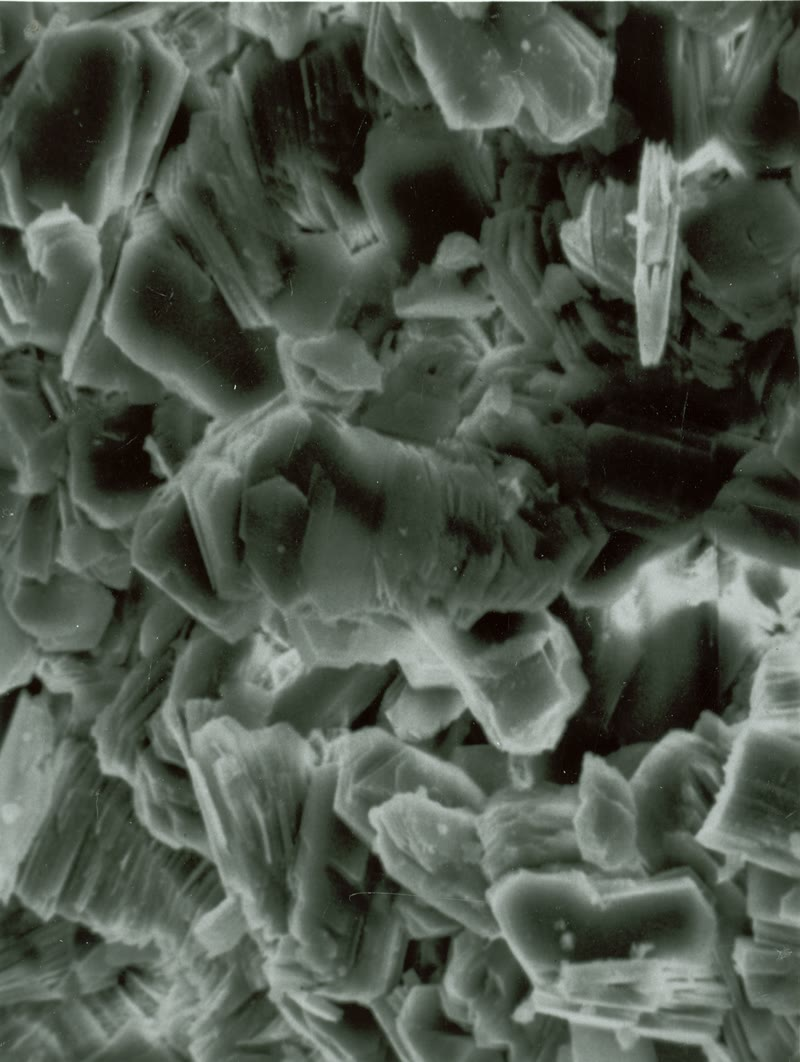
\includegraphics[width=\linewidth]{images/book3/b1-kaolinite-sem.jpg}

{\scriptsize De la \omterm{def:b1:weathering-clays:clay-mineral}{kaolinite} vue au microscope électronique à balayage~: des livres de
plaquettes hexagonales empilées développées dans les pores d'un grès du nord de l'Alaska
(grossissement environ 1340). U.S. Geological Survey, domaine public, via
Wikimedia Commons.\par}
\end{minipage}
\end{omfigure}
% ledger: biscaye:1965, usgs:clay-settings, pedron:stages, commons:kaolinite-sem

\emph{Les \omterm{def:b1:weathering-clays:laterite}{latérites}.} Là où l'\omterm{def:b1:weathering-clays:hydrolysis}{hydrolyse} atteint ses derniers degrés pendant longtemps,
le profil s'épaissit et son sommet concentre tout ce qui ne part pas.

\begin{definition}[Latérite]\label{def:b1:weathering-clays:laterite}
Une \emph{latérite}\index{laterite@latérite} est le produit riche en fer et en aluminium d'une
\omterm{def:b1:weathering-clays:hydrolysis}{hydrolyse} intense et prolongée sous des climats chauds et humides~: un
matériau rouge à brun, tendre ou induré, fait de \omterm{def:b1:weathering-clays:clay-mineral}{kaolinite} et d'oxydes et hydroxydes de fer,
avec de la gibbsite là où l'\omterm{def:b1:weathering-clays:hydrolysis-degree}{allitisation} est atteinte, d'où presque tous les cations alcalins
et alcalino-terreux et une grande part de la silice ont été retirés.
\end{definition}
% ledger: formoso:laterite, buchanan:laterite

Une \omterm{def:b1:weathering-clays:laterite}{latérite} assez riche en gibbsite ou en boehmite, les hydroxydes d'aluminium, est une
bauxite, le minerai des neuf dixièmes de l'aluminium~: l'\omterm{def:b1:weathering-clays:hydrolysis-degree}{allitisation} est l'étape qui
fait le minerai. La plupart des bauxites sont résiduelles, la roche dont tout sauf
l'alumine a été lessivé~; la plupart de celles faites de gibbsite se trouvent sous
les tropiques, et beaucoup sont probablement encore en formation.
% ledger: usgs:bauxite

\begin{history}[Un mot du terrain]
En 1807 Francis Buchanan, voyageant au Malabar, dans le sud de l'Inde, décrivit
un matériau plein de cavités et riche en ocres rouges et jaunes de fer, étalé
sur le granite en grandes masses. Extrait du sol il était si tendre qu'un
couteau le coupait, et les habitants le façonnaient en blocs~; à l'air il devenait vite
aussi dur que la brique, et durait mieux que toute brique qu'il avait vue. Les
langues locales l'appelaient pierre-brique~; il proposa le nom de \omterm{def:b1:weathering-clays:laterite}{latérite}, que la
géologie a gardé pour les produits rouges de l'altération tropicale.
\end{history}
% ledger: buchanan:laterite

\section{Altération des silicates et dioxyde de carbone}\label{sec:b1:weathering-clays:co2}

Les ions hydrogène de l'\omterm{def:b1:weathering-clays:hydrolysis}{hydrolyse} viennent surtout du dioxyde de carbone, donc les écrire
comme de l'acide carbonique montre ce que l'altération fait à l'air. Pour un silicate de calcium,
notée \ce{CaSiO3} par simplicité,
\[
  \ce{CaSiO3 + 2 CO2 + H2O -> Ca^2+ + 2 HCO3- + SiO2},
\]
et dans l'océan, où des organismes construisent des coquilles de carbonate de calcium,
\[
  \ce{Ca^2+ + 2 HCO3- -> CaCO3 + CO2 + H2O}.
\]

\begin{proposition}[Altération et dioxyde de carbone]\label{prop:b1:weathering-clays:co2}
(a) L'altération d'un silicate consomme deux moles de dioxyde de carbone, transformées en
bicarbonate, pour chaque mole de calcium ou de magnésium libérée~; quand le calcium
ou le magnésium est précipité sous forme de carbonate, l'une des deux retourne à l'air,
et une mole est stockée sous forme de roche carbonatée. (b) L'altération d'une roche carbonatée et la
précipitation de nouveau de son carbonate n'en stockent aucune.
\end{proposition}

\begin{proof}
(a) En additionnant les deux équations ci-dessus on obtient \ce{CaSiO3 + CO2 -> CaCO3 + SiO2}~:
un \ce{CO2} par calcium quitte l'air pour de bon~; la première équation seule
montre les deux consommés. Pour le magnésium il en va de même, avec \ce{Mg^2+} à la place de
\ce{Ca^2+}. (b) La dissolution de la calcite, \ce{CaCO3 + CO2 + H2O -> Ca^2+ + 2
HCO3-}, est exactement l'inverse de la précipitation~: la somme des deux est nulle.
\end{proof}

Avec un \omterm{def:b1:rock-forming-minerals:groups}{feldspath}, l'acide carbonique remplace les ions hydrogène de la
\cref{prop:b1:weathering-clays:feldspars}~: chaque \ce{H+} consommé est un
\ce{CO2} transformé en \ce{HCO3-}. L'anorthite d'un basalte ou d'un gabbro
consomme donc deux moles de dioxyde de carbone par mole en se transformant en \omterm{def:b1:weathering-clays:clay-mineral}{kaolinite},
\[
  \ce{CaAl2Si2O8 + 2 CO2 + 3 H2O -> Al2Si2O5(OH)4 + Ca^2+ + 2 HCO3-},
\]
et en stocke une à long terme. Le sodium et le potassium ne forment pas de carbonate sur le
fond marin, et le stockage à long terme se compte à partir du calcium et du magnésium
libérés.

Les rivières portent le bicarbonate à la mer, et leur chimie mesure le flux.
D'après la chimie des grandes rivières du monde, le dioxyde de carbone consommé par
l'altération des silicates continentaux a été estimé à \num{11.7e12} à
\qty{13.6e12}{mol} par an, soit environ 0.14 à 0.16 milliard de tonnes de carbone, dont
l'altération des basaltes à elle seule rend compte de 30 à \qty{35}{\percent}. Le flux est petit à côté
des échanges de carbone entre l'air, les océans et les êtres vivants, mais il
ne s'inverse pas~: sur des millions d'années c'est la principale façon dont le dioxyde de carbone
fourni par les volcans quitte l'atmosphère. Parce que l'altération va plus vite quand
il fait plus chaud et plus humide, elle lie le dioxyde de carbone de l'air au climat,
qui à son tour dépend du dioxyde de carbone par l'effet de serre~: une
rétroaction négative qui stabilise la température de la Terre à l'échelle des temps
géologiques, étudiée dans le volume de deuxième année.
% ledger: dessert:silicate-co2, whk:1981

\section{Exercices}

\begin{exercise}[$\star$]\label{exo:b1:weathering-clays:1}
En utilisant les rayons \ce{K+} \qty{1.38}{\angstrom}, \ce{Fe^2+} \qty{0.78}{\angstrom},
\ce{Fe^3+} \qty{0.645}{\angstrom} et \ce{Ti^4+} \qty{0.605}{\angstrom}, calculer
le \omterm{def:b1:weathering-clays:ionic-potential}{potentiel ionique} de chaque ion et nommer son domaine. Pourquoi un sol gorgé d'eau
perd-il son fer alors qu'un sol bien drainé le garde~?
% ledger: shannon:radii-b19
\end{exercise}

\begin{exercise}[$\star$]\label{exo:b1:weathering-clays:2}
Quatre fractions argileuses sont analysées aux rayons X en préparations orientées. A~: un pic à
\SI{14}{\angstrom}, déplacé à \SI{17}{\angstrom} par l'éthylène glycol et à
\SI{10}{\angstrom} par chauffage à \SI{400}{\celsius}. B~: un pic à
\SI{7}{\angstrom}, inchangé par le glycol, disparu après chauffage à
\SI{550}{\celsius}. C~: un pic à \SI{10}{\angstrom} qu'aucun traitement ne déplace. D~:
un pic à \SI{14}{\angstrom} qu'aucun traitement ne déplace. Identifier chaque \omterm{def:b1:rock-forming-minerals:mineral}{minéral}.
% ledger: usgs:clay-xrd
\end{exercise}

\begin{exercise}[$\star$]\label{exo:b1:weathering-clays:3}
Équilibrer, avec la \cref{met:b1:weathering-clays:balance}, l'\omterm{def:b1:weathering-clays:hydrolysis}{hydrolyse} de
l'orthose \ce{KAlSi3O8} en \omterm{def:b1:weathering-clays:clay-mineral}{kaolinite}. Quelle fraction de son potassium et de
son silicium part en solution~?
\end{exercise}

\begin{exercise}[$\star$]\label{exo:b1:weathering-clays:4}
(a) Quel volume de glace donnent \qty{10}{cm^3} d'eau à \qty{0}{\celsius}~?
(b) Dans quel intervalle de température la glace qui croît dans les fissures fend-elle la roche
le plus efficacement, et pourquoi ni un gel plus léger ni un gel plus dur ne fait-il aussi bien~?
(c) Un cube de granite de côté \qty{1}{m} est fendu par le gel en cubes de côté
\qty{1}{cm}~: de quel facteur sa surface a-t-elle crû~?
% ledger: usgs:water-density, iapws:ice-density, wh85:frost
\end{exercise}

\begin{exercise}[$\star\star$]\label{exo:b1:weathering-clays:5}
Calculer la surface spécifique de grains de \omterm{def:b1:rock-forming-minerals:groups}{feldspath} de masse volumique
\qty{2600}{kg.m^{-3}}, traités comme des cubes, pour des tailles de \qty{1}{cm}, \qty{1}{mm}
et \qty{1}{\micro m}. Pourquoi la taille des grains compte-t-elle tant pour la vitesse de
l'\omterm{def:b1:weathering-clays:weathering}{altération chimique}, et pourquoi l'\omterm{def:b1:weathering-clays:weathering}{altération physique} accélère-t-elle l'\omterm{def:b1:weathering-clays:weathering}{altération
chimique}~?
\end{exercise}

\begin{exercise}[$\star\star$]\label{exo:b1:weathering-clays:6}
Une tonne d'albite \ce{NaAlSi3O8} (\qty{262.22}{g.mol^{-1}}) est transformée en
\omterm{def:b1:weathering-clays:clay-mineral}{kaolinite} (\qty{258.16}{g.mol^{-1}}). Calculer la masse de \omterm{def:b1:weathering-clays:clay-mineral}{kaolinite} formée, la
masse de silice exportée, comptée comme \ce{SiO2} (\qty{60.08}{g.mol^{-1}}), et la
masse de sodium exportée.
% ledger: webmineral:clays-b19, ciaaw:Na
\end{exercise}

\begin{exercise}[$\star\star$]\label{exo:b1:weathering-clays:7}
Un granite contient, en masse, \qty{0.30}{\percent} de \ce{TiO2}, \qty{3.5}{\percent}
de \ce{Na2O}, \qty{72}{\percent} de \ce{SiO2} et \qty{14}{\percent} de \ce{Al2O3}~; sa
saprolite contient \qty{0.60}{\percent} de \ce{TiO2}, \qty{0.35}{\percent}
de \ce{Na2O}, \qty{60}{\percent} de \ce{SiO2} et \qty{27}{\percent} de \ce{Al2O3}.
En prenant le titane comme immobile, trouver la masse de saprolite laissée par un kilogramme de
granite et la fraction de sodium, de silicium et d'aluminium perdue. Quel degré
d'\omterm{def:b1:weathering-clays:hydrolysis}{hydrolyse} est en cours~?
\end{exercise}

\begin{exercise}[$\star\star$]\label{exo:b1:weathering-clays:8}
Avec la \cref{prop:b1:weathering-clays:layer-charge}, calculer la charge de feuillet de
la pyrophyllite \ce{Al2Si4O10(OH)2}, de la muscovite \ce{KAl2(Si3Al)O10(OH)2} sans
son potassium, du feuillet de beidellite \ce{Al2(Si_{3.5}Al_{0.5})O10(OH)2} et
d'un feuillet de montmorillonite \ce{(Al_{1.67}Mg_{0.33})Si4O10(OH)2}. Lesquels peuvent
gonfler, et pourquoi~?
% ledger: webmineral:clays-b19
\end{exercise}

\begin{exercise}[$\star\star$]\label{exo:b1:weathering-clays:9}
La forstérite \ce{Mg2SiO4} s'altère par
\ce{Mg2SiO4 + 4 CO2 + 4 H2O -> 2 Mg^2+ + 4 HCO3- + H4SiO4}. (a) Vérifier
l'équation. (b) Pour une tonne de forstérite, calculer le dioxyde de carbone consommé et
le dioxyde de carbone stocké à long terme d'après la
\cref{prop:b1:weathering-clays:co2}. (c) Que donnerait le même calcul
pour une tonne de calcite~?
% ledger: ciaaw:Mg, ciaaw:Si, ciaaw:O, ciaaw:C
\end{exercise}

\begin{exercise}[$\star\star\star$]\label{exo:b1:weathering-clays:10}
(a) Entre quels rayons un ion de charge 3 est-il un hydrolysat~? (b) Le bore,
\ce{B^3+}, a un rayon de \qty{0.27}{\angstrom}~: sous quelle forme voyage-t-il
dans l'eau~? (c) \ce{Mn^2+} a un rayon de \qty{0.83}{\angstrom}, \ce{Mn^4+} de
\qty{0.53}{\angstrom}. Expliquer pourquoi des \omterm{def:b1:layered-earth:layers}{croûtes} noires d'oxyde de manganèse se forment là où
une eau de source, pauvre en oxygène, débouche à l'air. (d) Pourquoi le silicium ne peut-il
être ni totalement lessivé ni totalement conservé~?
% ledger: shannon:radii-b19, nomad:goldschmidt
\end{exercise}

\begin{exercise}[$\star\star\star$]\label{exo:b1:weathering-clays:11}
L'altération des silicates continentaux consomme \num{11.7e12} à
\qty{13.6e12}{mol} de dioxyde de carbone par an, dont \qty{4.08e12}{mol} issues des
basaltes. (a) Convertir l'intervalle en tonnes de carbone et de dioxyde de carbone par
an. (b) Quelle part prennent les basaltes~? (c) Si tout cela provenait de silicates de calcium et de
magnésium, combien de carbone serait stocké à long terme chaque
année~? Pourquoi le chiffre réel à long terme est-il plus petit~?
% ledger: dessert:silicate-co2, ciaaw:C, ciaaw:O
\end{exercise}

\begin{exercise}[$\star\star\star$]\label{exo:b1:weathering-clays:12}
Trois fractions argileuses, débarrassées de quartz et d'oxydes de fer, sont analysées (pour
cent en masse)~: A, \ce{SiO2} \num{46.55} et \ce{Al2O3} \num{39.50}~; B, \ce{SiO2} 60 et
\ce{Al2O3} 25~; C, \ce{SiO2} 2 et \ce{Al2O3} 63 (\ce{SiO2}
\qty{60.08}{g.mol^{-1}}, \ce{Al2O3} \qty{101.96}{g.mol^{-1}}). Calculer le
rapport molaire Si/Al de chacune, identifier le degré d'\omterm{def:b1:weathering-clays:hydrolysis}{hydrolyse} qu'il enregistre, et
placer les trois sols sur une ligne du lessivage le moins intense au plus intense.
% ledger: webmineral:clays-b19, pedron:stages, formoso:laterite
\end{exercise}

\section{Problème~: Du granite à l'argile}

\begin{problem}[{Problème du week-end --- les feldspaths d'un granite et d'un gabbro, des
réactions équilibrées au dioxyde de carbone qu'emporte une rivière}]
\label{pb:b1:weathering-clays:1}
% values: calc/ch19.py; the river is invented (its numbers are of a realistic order)
Les \omterm{def:b1:rock-forming-minerals:groups}{feldspaths} sont l'albite \ce{NaAlSi3O8} (\qty{262.22}{g.mol^{-1}}, masse volumique
\qty{2.62}{g.cm^{-3}}) et l'anorthite \ce{CaAl2Si2O8}
(\qty{278.20}{g.mol^{-1}}, masse volumique \qty{2.75}{g.cm^{-3}}). La \omterm{def:b1:weathering-clays:clay-mineral}{kaolinite}
\ce{Al2Si2O5(OH)4} a pour masse molaire \qty{258.16}{g.mol^{-1}} et pour masse volumique
\qty{2.6}{g.cm^{-3}}~; la gibbsite \ce{Al(OH)3}, \qty{78.00}{g.mol^{-1}}. Prendre
\ce{SiO2} \qty{60.08}{g.mol^{-1}}, \ce{CO2} \qty{44.01}{g.mol^{-1}}, \ce{HCO3-}
\qty{61.02}{g.mol^{-1}}, Na \num{22.99} et Ca \qty{40.08}{g.mol^{-1}}.
% ledger: hom:albite, hom:anorthite, webmineral:clays-b19, ciaaw:Na, ciaaw:Ca, ciaaw:C, ciaaw:O, ciaaw:H

\medskip
\noindent\textbf{Partie I --- Les réactions.}
\begin{enumerate}
  \item Équilibrer l'\omterm{def:b1:weathering-clays:hydrolysis}{hydrolyse} de l'albite en \omterm{def:b1:weathering-clays:clay-mineral}{kaolinite}.
  \item Équilibrer l'\omterm{def:b1:weathering-clays:hydrolysis}{hydrolyse} de l'anorthite en \omterm{def:b1:weathering-clays:clay-mineral}{kaolinite}. Qu'a-t-elle de
        particulier~?
  \item Équilibrer l'\omterm{def:b1:weathering-clays:hydrolysis}{hydrolyse} de l'anorthite en gibbsite.
  \item Équilibrer l'\omterm{def:b1:weathering-clays:hydrolysis}{hydrolyse} de l'albite en beidellite
        \ce{Na_{0.5}Al2(Si_{3.5}Al_{0.5})O10(OH)2}, et vérifier l'hydrogène.
  \item Réécrire les deux premières réactions avec l'acide carbonique comme source
        des ions hydrogène~: \ce{CO2 + H2O -> H+ + HCO3-}.
  \item Lesquelles de ces réactions sont de la \omterm{def:b1:weathering-clays:hydrolysis-degree}{bisiallitisation}, de la \omterm{def:b1:weathering-clays:hydrolysis-degree}{monosiallitisation} et
        de l'\omterm{def:b1:weathering-clays:hydrolysis-degree}{allitisation}~?
\end{enumerate}

\medskip
\noindent\textbf{Partie II --- Ce qui reste, ce qui part.}
\begin{enumerate}[resume]
  \item Combien de moles y a-t-il dans une tonne d'albite, et dans une tonne
        d'anorthite~?
  \item Calculer la masse de \omterm{def:b1:weathering-clays:clay-mineral}{kaolinite} formée à partir d'une tonne de chacune.
  \item Calculer les masses de silice (comme \ce{SiO2}), de sodium et de calcium
        exportées en solution.
  \item Calculer le volume d'une tonne de chaque \omterm{def:b1:rock-forming-minerals:groups}{feldspath} et de la \omterm{def:b1:weathering-clays:clay-mineral}{kaolinite} qu'il
        donne. De quelle fraction le volume de solide diminue-t-il~?
  \item Une saprolite garde la forme de la roche qu'elle remplace. Qu'est-ce qui remplit
        l'espace laissé dans un granite altéré riche en albite~? Pourquoi un gabbro
        altéré riche en anorthite reste-t-il plus dense~?
  \item Avec le diagramme du \omterm{def:b1:weathering-clays:ionic-potential}{potentiel ionique}, expliquer lesquels des éléments des
        deux \omterm{def:b1:rock-forming-minerals:groups}{feldspaths} partent et lesquels restent.
\end{enumerate}

\medskip
\noindent\textbf{Partie III --- Le dioxyde de carbone.}
\begin{enumerate}[resume]
  \item Combien de moles, et combien de kilogrammes, de dioxyde de carbone sont consommés
        quand une tonne d'albite se transforme en \omterm{def:b1:weathering-clays:clay-mineral}{kaolinite}~?
  \item Même question pour une tonne d'anorthite.
  \item Quelle masse de bicarbonate est exportée par l'anorthite~?
  \item Qu'advient-il de ce bicarbonate dans l'océan~? Quelle part du dioxyde de carbone
        consommé retourne à l'air~?
  \item Pourquoi aucun stockage à long terme n'est-il compté pour le sodium de l'albite~?
  \item Comparer avec la dissolution d'une tonne de calcite suivie de sa
        précipitation.
\end{enumerate}

\medskip
\noindent\textbf{Partie IV --- Une rivière.}
\begin{enumerate}[resume]
  \item Une rivière draine \qty{50000}{km^2} de granite et de gneiss, avec un débit
        moyen de \qty{200}{m^3.s^{-1}}~; le bicarbonate qu'elle transporte issu de
        l'altération des silicates est de \qty{0.3}{mmol.L^{-1}}. Calculer le flux annuel
        de ce bicarbonate, en moles, et par kilomètre carré.
  \item L'exprimer en moles d'anorthite dont l'altération en \omterm{def:b1:weathering-clays:clay-mineral}{kaolinite}
        l'apporterait, puis en tonnes d'anorthite par an et par kilomètre
        carré.
  \item Si la roche contient l'équivalent de \qty{20}{\percent}
        d'anorthite et a pour masse volumique \qty{2700}{kg.m^{-3}}, à quelle vitesse, en
        mètres par million d'années, la roche fraîche est-elle consommée~?
  \item Quelle quantité de dioxyde de carbone cette rivière retire-t-elle de l'air pour de bon
        chaque année~?
  \item Pourquoi la vitesse de la question 21 est-elle une borne inférieure de l'abaissement de
        la surface du sol~?
  \item En kilogrammes, à trois chiffres, quelle quantité de dioxyde de carbone est retirée
        pour de bon par l'altération d'une tonne d'anorthite~?
\end{enumerate}
\end{problem}
